\chapter{Backend Mystery} 

\section{MTV framework}
\section{Models and Database}
\section{Django Template Language}
\section{Request-Response Flow}

How Teakwood process a request from user?
\begin{figure}[htb]
\centering
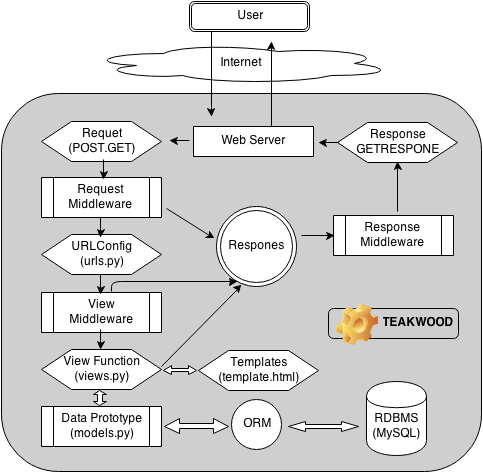
\includegraphics[scale=0.8]{./http_request_response}
\caption{<Caption here>}
\label{fig:label} % insert suitable label, this is used to refer to a fig from within the text as shown above
\end{figure}

\section{Lose Coupling}
\section{Powerful Admin}

